\PassOptionsToPackage{unicode=true}{hyperref} % options for packages loaded elsewhere
\PassOptionsToPackage{hyphens}{url}
%
\documentclass[]{article}
\usepackage{lmodern}
\usepackage{amssymb,amsmath}
\usepackage{ifxetex,ifluatex}
\usepackage{fixltx2e} % provides \textsubscript
\ifnum 0\ifxetex 1\fi\ifluatex 1\fi=0 % if pdftex
  \usepackage[T1]{fontenc}
  \usepackage[utf8]{inputenc}
  \usepackage{textcomp} % provides euro and other symbols
\else % if luatex or xelatex
  \usepackage{unicode-math}
  \defaultfontfeatures{Ligatures=TeX,Scale=MatchLowercase}
\fi
% use upquote if available, for straight quotes in verbatim environments
\IfFileExists{upquote.sty}{\usepackage{upquote}}{}
% use microtype if available
\IfFileExists{microtype.sty}{%
\usepackage[]{microtype}
\UseMicrotypeSet[protrusion]{basicmath} % disable protrusion for tt fonts
}{}
\IfFileExists{parskip.sty}{%
\usepackage{parskip}
}{% else
\setlength{\parindent}{0pt}
\setlength{\parskip}{6pt plus 2pt minus 1pt}
}
\usepackage{hyperref}
\hypersetup{
            pdfborder={0 0 0},
            breaklinks=true}
\urlstyle{same}  % don't use monospace font for urls
\usepackage{longtable,booktabs}
% Fix footnotes in tables (requires footnote package)
\IfFileExists{footnote.sty}{\usepackage{footnote}\makesavenoteenv{longtable}}{}
\usepackage{graphicx,grffile}
\makeatletter
\def\maxwidth{\ifdim\Gin@nat@width>\linewidth\linewidth\else\Gin@nat@width\fi}
\def\maxheight{\ifdim\Gin@nat@height>\textheight\textheight\else\Gin@nat@height\fi}
\makeatother
% Scale images if necessary, so that they will not overflow the page
% margins by default, and it is still possible to overwrite the defaults
% using explicit options in \includegraphics[width, height, ...]{}
\setkeys{Gin}{width=\maxwidth,height=\maxheight,keepaspectratio}
\setlength{\emergencystretch}{3em}  % prevent overfull lines
\providecommand{\tightlist}{%
  \setlength{\itemsep}{0pt}\setlength{\parskip}{0pt}}
\setcounter{secnumdepth}{0}
% Redefines (sub)paragraphs to behave more like sections
\ifx\paragraph\undefined\else
\let\oldparagraph\paragraph
\renewcommand{\paragraph}[1]{\oldparagraph{#1}\mbox{}}
\fi
\ifx\subparagraph\undefined\else
\let\oldsubparagraph\subparagraph
\renewcommand{\subparagraph}[1]{\oldsubparagraph{#1}\mbox{}}
\fi

% set default figure placement to htbp
\makeatletter
\def\fps@figure{htbp}
\makeatother


\date{}

\begin{document}

\hypertarget{header-n8510}{%
\section{Exercice 1 :}\label{header-n8510}}

\(f\) est la fonction définie sur \(\mathbb{R}\) par :
\(f(x) = xe^{\frac{-x^2}{2}}\).\\
On note \(\mathscr{C}\) la courbe représentative de la fonction \(f\)
dans un repère orthonormé du plan.

\hypertarget{header-n8512}{%
\subsection{1. Étude de la fonction}\label{header-n8512}}

\hypertarget{header-n8513}{%
\subsubsection{\texorpdfstring{a) étudier la parité de la fonction
\(f\)}{a) étudier la parité de la fonction f}}\label{header-n8513}}

On sait, par définition qu'une fonction \(f\) est paire si et seulement
si pour tout \(x\) dans \(\mathbb{R}\), \(f(-x) = f(x)\), et qu'une
fonction est impaire si et seulement si pour tout \(x\) dans
\(\mathbb{R}\), \(f(-x) = -f(x)\).\\
 ~\\
Or, on sait que \(f(-x) = -xe^{\frac{-x^2}{2}} = -f(x)\), on peut donc
dire que la fonction \(f\) est impaire.\\

\hypertarget{header-n8515}{%
\subsubsection{\texorpdfstring{b) Établir le tableau de variations de
\(f\) sur l'intervalle
\([0; +\infty[\).}{b) Établir le tableau de variations de f sur l'intervalle {[}0; +\textbackslash{}infty{[}.}}\label{header-n8515}}

On calcule d'abord \(f'\) :\\
 ~\\
On pose \(u(x) = x\), \(u'(x) = 1\); \(v(x) = \dfrac{-x^2}{2}\),
\(v'(x) = -x\)\\
\[
\begin{array}{rl}
        f'(x) &= u'(x)\left(e^v\right)(x) + u(x)\left(e^v\right)'(x)\\
              &= 1\left(e^{\frac{-x^2}{2}}\right) + x\left(-xe^{\frac{-x^2}{2}}\right)\\
              &= e^{\frac{-x^2}{2}} - x^2e^{\frac{-x^2}{2}}\\
              &= e^{\frac{-x^2}{2}}\left(1-x^2\right)\\
    \end{array}
\]
On cherche à déterminer le signe de \(1-x^2\) sur \(\mathbb{R}^+\), or
\(1-x^2>0 \iff x^2 < 1 \iff x < 1\)

\begin{longtable}[]{@{}cccc@{}}
\toprule
\(x\) & \(0\) & \(1\) & \(+\infty\)\tabularnewline
\midrule
\endhead
signe de \(e^{\frac{-x^2}{2}}\) & \(+\) & \(+\) & \(+\)\tabularnewline
signe de \(1-x^2\) & \(-\) & \(+\) & \(-\)\tabularnewline
signe de \(f'(x)\) & \(-\) & \(+\) & \(-\)\tabularnewline
variations de \(f\) & \(\searrow\) & \(\nearrow\) &
\(\searrow\)\tabularnewline
\bottomrule
\end{longtable}

\hypertarget{header-n8545}{%
\subsubsection{\texorpdfstring{c) Déterminer une équation de la tangente
\(T_0\) à la courbe \(\mathscr{C}\) au point d'abscisse
\(0\).}{c) Déterminer une équation de la tangente T\_0 à la courbe \textbackslash{}mathscr\{C\} au point d'abscisse 0.}}\label{header-n8545}}

Une équation de la tangente est :
\[
\begin{array}{rll}
        y &=& f'(a)(x-a) + f(a)\\
          &=& \left(e^{\frac{-a^2}{2}}\left(1-a^2\right)\right)(x - a) + ae^{\frac{-x^2}{2}}\Big{|}_{a=0}\\
          &=& \left(e^{\frac{-(0)^2}{2}}\left(1-(0)^2\right)\right)(x - 0) + (0)e^{\frac{-x^2}{2}}\\
          &=& e^{0}(x - 0)\\
        y &=& x
    \end{array}
\]
\hypertarget{header-n8548}{%
\subsubsection{\texorpdfstring{d) Étudier la convexité de \(f\) et
déterminer les éventuels points
d'inflextion}{d) Étudier la convexité de f et déterminer les éventuels points d'inflextion}}\label{header-n8548}}

Pour étudier la convexité de \(f\), on cherche le signe de \(f''(x)\).

On pose :
\[
\begin{array}{c}
        u(x) = e^{\frac{-x^2}{2}}\\
        u'(x) = -xe^{\frac{-x^2}{2}}\\
        \\
        v(x) = 1-x^2\\
        v'(x) = -2x\\
    \end{array}

On sait que :
\]
\[f'(x) = u(x)v(x)\]

On en déduit que :
\[
\begin{array}{rll}
        f''(x) &= u'(x)v(x) + u(x)v'(x)\\
               &= -xe^{\frac{-x^2}{2}}\left(1-x^2\right) - 2xe^{\frac{-x^2}{2}}\\
               &= e^{\frac{-x^2}{2}}\left(-x\left(1-x^2\right) - 2x\right)\\
               &= e^{\frac{-x^2}{2}}\left(x^3 - 3x \right)\\
               &= e^{\frac{-x^2}{2}}\left(x\left(x^2 - 3\right)\right)\\
               &= xe^{\frac{-x^2}{2}}\left(x^2 - 3\right)
    \end{array}
\]
On sait que la fonction exponentielle est positive \(\mathbb{R}\). On
peut donc dire que \(e^{\frac{-x^2}{2}} > 0\).\\
On cherche le signe de \((x^2 - 3)\) :
\(x^2 - 3 > 0 ⟺ x^2 > 3 ⟺ -\sqrt{3} > x > \sqrt{3}\)

On à donc :

\begin{longtable}[]{@{}cccccccl@{}}
\toprule
\(x\) & \(-\infty\) & \(-\sqrt{3}\) & \(-1\) & \(0\) & \(1\) &
\(\sqrt{3}\) & \(+\infty\)\tabularnewline
\midrule
\endhead
signe de \(xe^{\frac{-x^2}{2}}\) & \(-\) & \(-\) & \(-\) & \(0\) & \(+\)
& \(+\) & \(+\)\tabularnewline
signe de \(x^2-3\) & \(+\) & \(0\) & \(-\) & \(-\) & \(-\) & \(0\) &
\(+\)\tabularnewline
signe de \(f''(x)\) & \(-\) & \(0\) & \(+\) & \(0\) & \(-\) & \(0\) &
\(+\)\tabularnewline
\bottomrule
\end{longtable}

On voit donc que \(f\) est concave sur \(]-\infty; -\sqtr{3}]\), puis
convexe sur \([-\sqrt{3}; 0]\), concave sur \([]\)

\begin{figure}
  \centering
  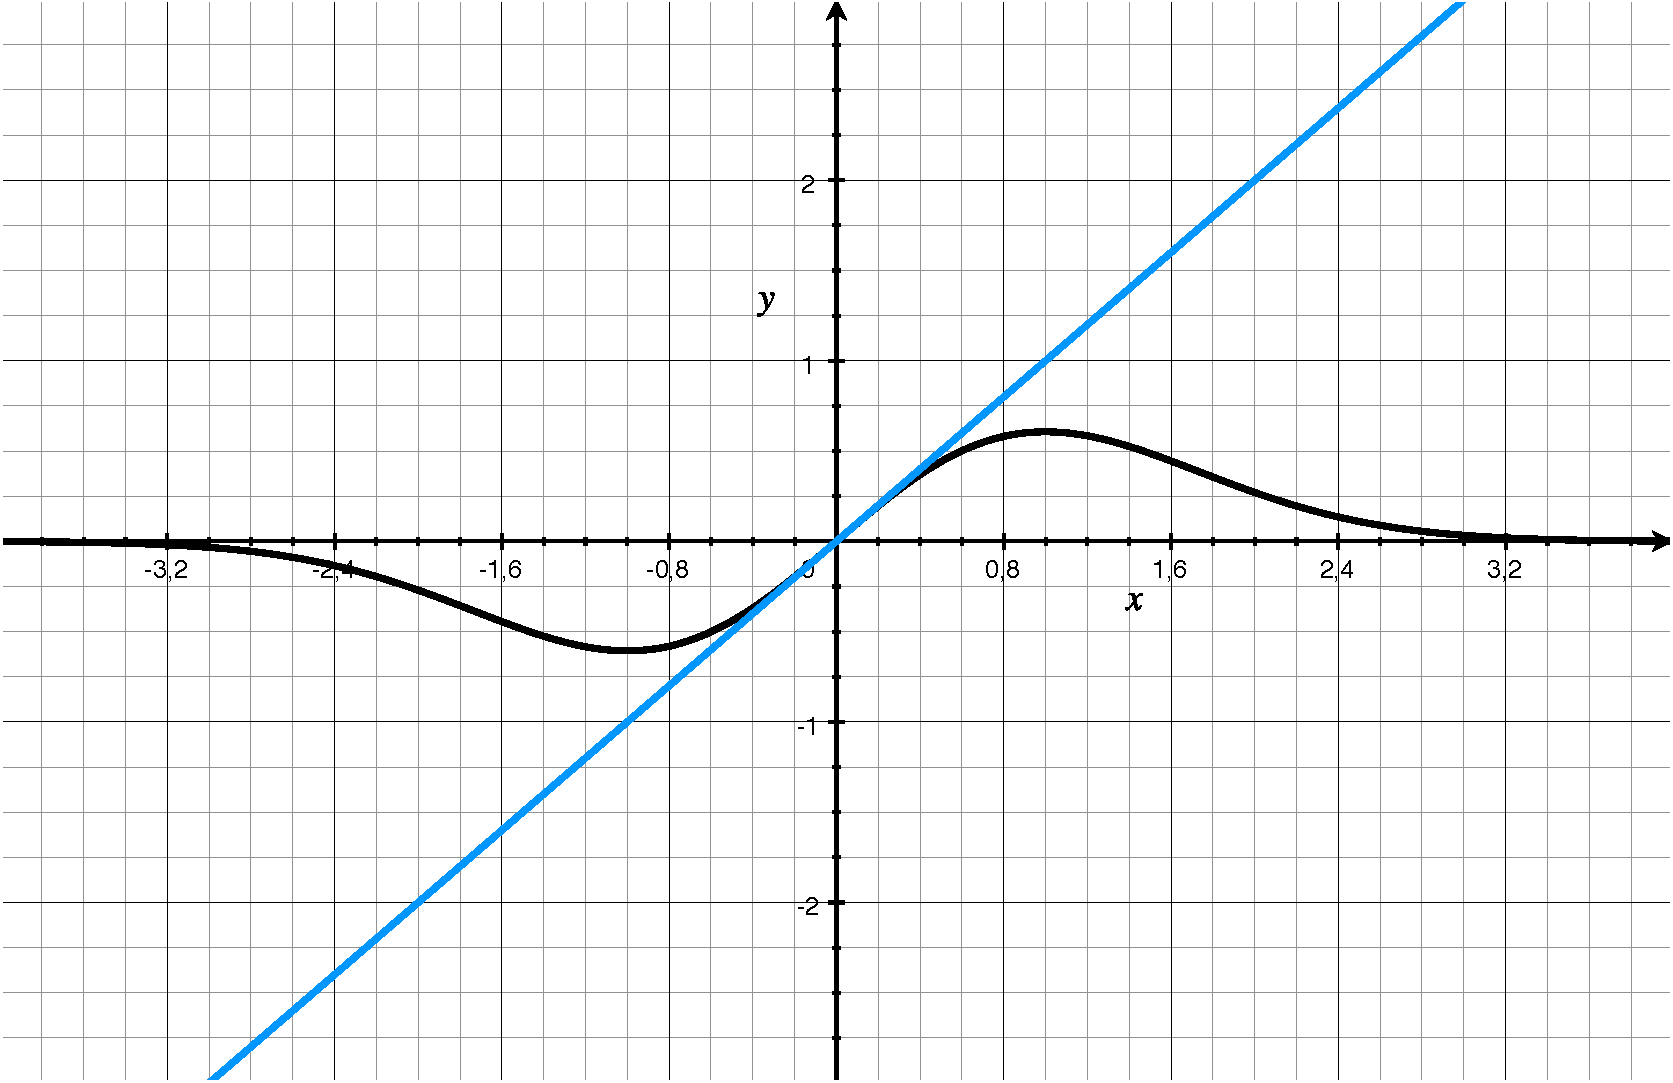
\includegraphics{Graphique.png}
  \caption{}
\end{figure}

\end{document}
